
As shown in homework D.3, the equations of motion for the mass-spring-damper are given by 
\begin{equation}\label{eq:soln_d5_1}
m\ddot{z} + b\dot{z} + kz = F 
\end{equation}
These equations are linear and do not require a linearization step prior to finding the corresponding transfer function.
Taking the Laplace transform of Equation~\eqref{eq:soln_d5_1} and setting all initial conditions to zero we get
\[
(ms^2 + bs + k) Z(s) = F(s).
\]
Solving for $Z(s)$ and putting the transfer function in monic form gives
\begin{equation}\label{eq:soln_d5_2}
Z(s) = \left(\frac{\frac{1}{m}}{s^2 + \frac{b}{m}s + \frac{k}{m}}\right) F(s).
\end{equation}
where the expression in the parenthesis is the transfer function from $F$ to $z$. The block diagram associated with Equation~\eqref{eq:soln_d5_2} is shown in Figure~\ref{fig:hw_mass_block_diagram}
\begin{figure}[htbp]
   \centering
   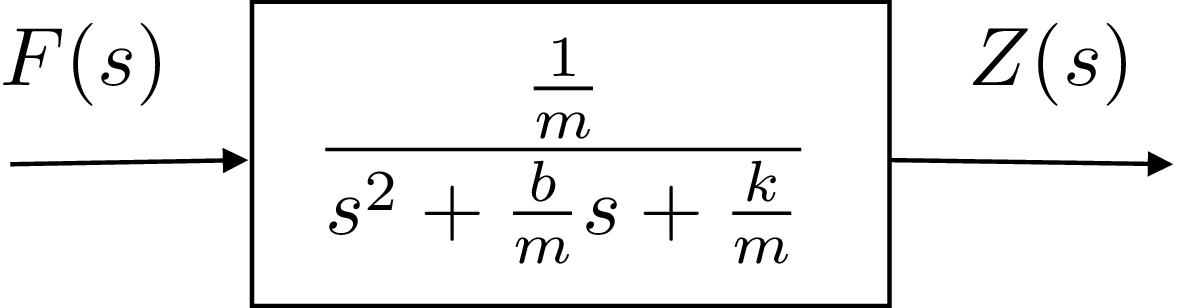
\includegraphics[width=0.4\textwidth]{6_design_studies/figures/hw_mass_block_diagram.pdf}
   \caption{A block diagram of the mass spring damper system.}
   \label{fig:hw_mass_block_diagram}
\end{figure} 
